\documentclass[11pt,halfparskip]{scrartcl}
\usepackage{amsmath}
\usepackage{booktabs}
\usepackage[T1]{fontenc}
\usepackage{graphicx}
\usepackage{natbib}

\bibliographystyle{agufull08}

\newcommand{\changefont}[3]{\fontfamily{#1} \fontseries{#2} \fontshape{#3} \selectfont}

%% diverser Plunder
\renewcommand{\refname}{Literature}
%\newcommand{\tnoocomment}[1]{\marginpar{\psshadowbox[framearc=0.3,shadowsize=2pt]{\footnotesize #1}}}
\newcommand{\tnoocomment}[1]{\marginpar{\fbox{\footnotesize #1}}}
\newcommand{\tinu}[1]{\marginpar{\fbox{\footnotesize #1}}}
\newcommand{\todo}[1]{\fbox{#1}}
\newcommand{\idea}[1]{\marginpar{\fbox{\parbox{2.2cm}{\tiny #1}}}}

%% commands to facilitate units and temperature
\newcommand{\unit}[1]{\ensuremath{\,\mathrm{#1}}}
\newcommand{\s}[1]{\ensuremath{\,\mathrm{#1}}}
\newcommand{\cels}[1]{\ensuremath{#1^{\circ}\,\mathrm{C}}}


\newcommand{\hbe}{\hat{\mathbf{e}}}
%\newcommand{\define}[1]{{\textbf{#1}}\marginpar{\psshadowbox[framearc=0.3,shadowsize=2pt]{\footnotesize #1}}}
\newcommand{\define}[1]{{\textbf{#1}}\marginpar{\fbox{\footnotesize #1}}}
\newcommand{\epsdot}{\dot{\varepsilon}}
\newcommand{\bsigma}{\mbox{\boldmath$\sigma$\unboldmath}}
\newcommand{\bepsdot}{\mbox{\boldmath$\epsdot$\unboldmath}}


% Some useful commands (from ELB)
\newcommand{\bD}{\mathbf{D}}
\newcommand{\bd}{\mathbf{d}}
\newcommand{\bbf}{\mathbf{f}}
\newcommand{\bF}{\mathbf{F}}
\newcommand{\bg}{\mathbf{g}}
\newcommand{\bn}{\mathbf{n}}
\newcommand{\bq}{\mathbf{q}}
\newcommand{\bT}{\mathbf{T}}
\newcommand{\bu}{\mathbf{u}}
\newcommand{\bU}{\mathbf{U}}
\newcommand{\bv}{\mathbf{v}}
\newcommand{\bw}{\mathbf{w}}

\newcommand{\ddx}[1]{\ensuremath{\frac{\partial #1}{\partial x}}}
\newcommand{\ddy}[1]{\ensuremath{\frac{\partial #1}{\partial y}}}
\newcommand{\ddz}[1]{\ensuremath{\frac{\partial #1}{\partial z}}}
\newcommand{\ddt}[1]{\ensuremath{\frac{\partial #1}{\partial t}}}

\newcommand{\DDt}[1]{\ensuremath{\frac{d #1}{d t}}}

\newcommand{\Div}{\nabla\cdot}
\newcommand{\eps}{\epsilon}
\newcommand{\grad}{\nabla}
\newcommand{\half}{\frac{1}{2}}
\newcommand{\trace}{\operatorname{tr}}

\newcommand{\rinv}{\frac{1}{r}}
\newcommand{\ar}{r^{-1}\alpha}
\newcommand{\stress}{\ensuremath{\text{\Large$\sigma$\normalsize}}}
\newcommand{\devstress}{\ensuremath{\text{\Large$\tau$\normalsize}}}


% ---------------------------------------------------------------------------------------
% definition of header and footer
% ---------------------------------------------------------------------------------------

\usepackage[automark,headsepline,footsepline]{scrpage2}
\clearscrheadings	
\ihead{Glacier Dynamics}
\ohead{McCarthy Summer School 2016}
\cfoot{\pagemark}
\setkomafont{pagehead}{\normalfont}
\setkomafont{pagenumber}{\normalfont\rmfamily}




% ---------------------------------------------------------------------------------------
% Koma-Script - Settings
% ---------------------------------------------------------------------------------------
\addtokomafont{caption}{\small}
\setkomafont{captionlabel}{\sffamily\bfseries}
% \setkomafont{caption}{\sffamily}
\setcapindent{1em}

\pagestyle{scrheadings}



\begin{document}
\title{Dynamics of Glaciers\\[.5em]
\rule[1.em]{\textwidth}{2pt}
\subtitle{McCarthy Summer School 2016}}

\date{}

\author{
  \small Andy Aschwanden\\[-.5em] 
  \small Geophysical Institute\\[-.5em] 
  \small University of Alaska Fairbanks, USA}


\maketitle

\textbf{Note}: This script is largely based on the \emph{Physics of
Glaciers I} lecture notes by Martin L\"uthi and Martin Funk, ETH
Zurich, Switzerland and \cite{GreveBlatter_disg}.

\vspace{1em}

\section{Flow relation for polycrystalline ice}
\label{sec:flow-law-ice}

The most widely used flow relation for glacier ice is
\citep{Glen1955,Steinemann1954}
%  
\begin{equation}
  \label{eq:Glen} \epsdot_{ij} = A \tau^{n-1}\sigma^{(d)}_{ij}.
\end{equation}
%
with $n\sim 3$, and where $\epsdot_{ij}$ and $\sigma^{(d)}_{ij}$ are
the strain rate tensor and the deviatoric stress tensor, respectively.
The rate factor $A = A(T)$ depends on temperature and other parameters
like water content, impurity content and crystal size.  The quantity
$\tau$ is the second invariant of the deviatoric stress tensor.
%
Several properties of Equation (\ref{eq:Glen}) are noteworthy:
\begin{itemize}
\item Elastic effects are neglected.  This is reasonable if processes on the
  time scale of days and longer are considered. But elastic effects are relevant to understand tidal flexure of ice shelves.
\item Stress and strain rate are collinear, i.e.~a shear stress leads to
  shearing strain rate, a compressive stress to a compressive strain rate, and
  so on.
\item Only deviatoric stresses lead to deformation rates, isotropic pressure
  alone cannot induce deformation. Ice is an \emph{incompressible} material
  (no volume change, except for elastic compression).  This is expressed as
  \[
  \epsdot_{ii} = 0 \qquad \Longleftrightarrow \qquad
  \frac{\partial v_x}{\partial x} + \frac{\partial v_y}{\partial y} +
  \frac{\partial v_z}{\partial z} = 0
  \]
\item A \emph{Newtonian viscous fluid}, like water, is characterized by
  the \emph{viscosity} $\eta$
  \begin{equation}
    \label{eq:viscosity-newtonian}
  \epsdot_{ij} = \frac{1}{2\eta} \sigma^{(d)}_{ij}.
  \end{equation}
  By comparison with Equation (\ref{eq:Glen}) we find that viscosity of
  glacier ice is
  \[
  \eta=\frac{1}{2A\tau^{n-1}}.
  \]

\item Polycrystalline glacier ice is a \emph{viscous fluid} with a
  \textbf{stress dependent viscosity} (or, equivalently, a strain rate
  dependent viscosity).  Such a material is called a \emph{non-Newtonian
    fluid}, or more specifically a \emph{power-law fluid}.
\item Polycrystalline glacier ice is treated as an \emph{isotropic fluid}. No
  preferred direction (due to crystal orientation fabric) appears in the flow
  relation.  This is a crude approximation to reality, since glacier ice
  usually is anisotropic, although to varying degrees.
  
%   This is approximately true for the major parts of glaciers due to ongoing
%   recrystallization.  The ice near bedrock is usually highly anisotropic,
%   especially in polar ice sheets.
\end{itemize}


Many alternative flow relations have been proposed that take into account the
compressibility of firn at low density,
% \citep[][e.g.]{Gagliardini&Meyssonnier1997},
the anisotropic nature of ice, microcracks and damaged ice,
% \citep{Pralong&al2006},
the water content, impurities and different grain sizes.  Glen's flow law is
still widely used because of its simplicity and ability to approximately
describe most processes relevant to glacier dynamics at large scale.

\subsection{Inversion of the flow relation}
\label{sec:invers-flow-relat}

The flow relation of Equation (\ref{eq:Glen}) can be inverted so that stresses
are expressed in terms of strain rates.  Multiplying equation (\ref{eq:Glen})
with itself gives
%
\begin{align}
  \qquad \qquad\epsdot_{ij}\epsdot_{ij} & = A^2 \tau^{2(n-1)}\sigma^{(d)}_{ij}\sigma^{(d)}_{ij}
  \qquad \qquad (\text{multiply by }\frac{1}{2}) \notag\\
  \underbrace{\frac{1}{2}\epsdot_{ij}\epsdot_{ij}}_{\dot{\epsilon}^2} &
  = A^2
  \tau^{2(n-1)}\underbrace{\frac{1}{2}\sigma^{(d)}_{ij}\sigma^{(d)}_{ij}}_{\tau^2}
  \notag
\end{align}
%
where we have used the definition for the \emph{effective strain rate}
$\dot{\epsilon} = \epsdot_e$, in
analogy to the \emph{effective shear stress} $\tau = \sigma_e$
%
\begin{equation}
  \label{eq:epsdot-e}
  \dot{\epsilon} = \sqrt{\frac{1}{2}\epsdot_{ij}\epsdot_{ij}}\,.
\end{equation}
%
This leads to a relation between tensor invariants
%
\begin{equation}
  \label{eq:Glen-invariants}
  \dot{\epsilon}  =  A\tau^n\,. 
\end{equation}
%
Coincidentally this is also the equation to describe simple shear, the most
important part of ice deformation in glaciers
%
\begin{equation}
  \label{eq:Glen-simple-shear}
  \dot{\epsilon}_{xz}  =  A\sigma^{(d)}_{xz} {}^n\,. 
\end{equation}
%
Now we can invert the flow relation Equation (\ref{eq:Glen})
%
\begin{align}
  \label{eq:Glen-inverse}
  \sigma^{(d)}_{ij} &= A^{-1}\tau^{1-n} \,\epsdot_{ij} \notag\\
  \sigma^{(d)}_{ij} &= A^{-1} A^\frac{n-1}{n}\, \dot{\epsilon}^{-\frac{n-1}{n}} \,\epsdot_{ij} \notag\\
  \sigma^{(d)}_{ij} &= A^{-\frac{1}{n}} \,\dot{\epsilon}^{-\frac{n-1}{n}}\, \epsdot_{ij}\,. 
\end{align}
%
The above relation allows us to calculate the stress state if the strain rates
are known (from measurements).  Notice that only deviatoric stresses can be
calculated. The mean stress (pressure) cannot be determined because of the
incompressibility of the ice.  Comparing Equation (\ref{eq:Glen-inverse}) with
(\ref{eq:viscosity-newtonian}) we see that the shear viscosity is
%
\begin{equation}
  \label{eq:viscosity-strainrate}
  \eta = \frac{1}{2}A^{-\frac{1}{n}} \,\dot{\epsilon}^{-\frac{n-1}{n}}.
\end{equation}
%
Polycrystalline ice is a \emph{strain rate softening}  material: viscosity
decreases as the strain rate increases.

Notice that the viscosity given in Equation (\ref{eq:viscosity-strainrate})
becomes infinite at very low strain rates, which of course is unphysical.  One
way to alleviate that problem is to add a small quantity $\eta_{o}$ to
obtain a \emph{finite viscosity}
%
\begin{equation}
  \label{eq:viscosity-strainrate-finite}
  \eta^{-1} = \left( \frac{1}{2}A^{-\frac{1}{n}} \,\dot{\epsilon}^{-\frac{n-1}{n}} \right)^{-1} + \eta_0^{-1}.
\end{equation}

\newpage
\section{Simple stress states}
\label{sec:simple-stress-states}

To see what Glen flow law of Equation (\ref{eq:Glen}) describes, we
investigate some simple, yet important stress states imposed on small samples
of ice, e.g.~in the laboratory.

\paragraph{a) Simple shear}

\begin{equation}
  \label{eq:simple-shear}
  \epsdot_{xz} = A (\sigma^{(d)}_{xy})^3 = A \sigma_{xy}^3
\end{equation}

This stress regime applies near the base of a glacier.

\paragraph{b) Unconfined uniaxial compression } along the vertical $z$-axis
%
\begin{align}
  \label{eq:uniaxial-unconfined}
  \sigma_{xx} &= \sigma_{yy} = 0\notag \\
  \sigma^{(d)}_{zz} &= \frac{2}{3} \sigma_{zz}; \qquad \sigma^{(d)}_{xx}= \sigma^{(d)}_{yy} =
  -\frac{1}{3} \sigma_{zz}\notag\\
  \epsdot_{xx} &= \epsdot_{yy} =
  -\frac{1}{2}\epsdot_{zz}
  = -\frac{1}{9}A \sigma_{zz}^3
  \notag\\
  \epsdot_{zz} &= \frac{2}{9}A \sigma_{zz}^3
\end{align}

This stress system is easy to investigate in laboratory experiments, and also
applies in the near-surface layers of an ice sheet.  The deformation rate is
only $22\unit{\%}$ of the deformation rate at a shear stress of equal
magnitude (Eq.~\ref{eq:simple-shear}).

\paragraph{c) Uniaxial compression} confined in the  $y$-direction
%
\begin{align}
  \label{eq:uniaxial-confined}
  \sigma_{xx} &= 0 ; \qquad \epsdot_{yy}=0;
  \qquad\epsdot_{xx} = -\epsdot_{zz}\notag \\
  \sigma^{(d)}_{yy} &= \frac{1}{3} \left(2\sigma_{yy} - \sigma_{zz} \right)=0 ;
  \qquad \sigma_{yy}= \frac{1}{2}\sigma_{zz} \notag\\
  \sigma^{(d)}_{xx} &= -\sigma^{(d)}_{zz} = -\frac{1}{3} \left(\sigma_{yy} + \sigma_{zz} \right)
  = -\frac{1}{2}\sigma_{zz}\notag\\
  \epsdot_{zz} &= \frac{1}{8}A \sigma_{zz}^3
\end{align}
%
This stress system applies in the near-surface layers of a valley glacier and
in an ice shelf occupying a bay.

\paragraph{d) Shear combined with unconfined uniaxial compression}
%
\begin{align}
  \label{eq:shear-uniaxial-confined}
  \sigma_{xx} &= \sigma_{yy} = \sigma_{xy} = \sigma_{yz} = 0\notag \\
  \sigma^{(d)}_{zz} &= \frac{2}{3} \sigma_{zz} = -2 \sigma^{(d)}_{xx} = -2 \sigma^{(d)}_{yy} \notag\\
  \tau^2 &= \frac{1}{3}\sigma_{zz}^2 + \sigma_{xz}^2 \notag \\
  \epsdot_{zz} &= -2\epsdot_{xx} =
  -2\epsdot_{yy} = \frac{2}{3} A \tau^2 \sigma_{zz} \notag\\
  \epsdot_{xz} &= A\tau^2 \sigma_{xz}
\end{align}
%
This stress configuration applies at many places in ice sheets.

\section{Field equations}
\label{sec:field-equations}

To calculate velocities in a glacier we have to solve \emph{field
  equations}. \index{Field equations} For a mechanical problem (e.g.~glacier
flow) we need the \emph{continuity of mass} \index{continuity of mass} and the
\emph{force balance equations}.  The \define{mass continuity} equation for a
compressible material of density $\rho$ is (in different notations)
%
\begin{subequations}
  \label{eq:mass-continuity}
\begin{align}
   \frac{\partial \rho}{\partial t} + \frac{\partial(\rho u)}{\partial x} +
    \frac{\partial(\rho v)}{\partial y} + \frac{\partial(\rho w)}{\partial z} &=0\\
  \frac{\partial \rho}{\partial t} + \mathbf{\nabla} \cdot (\rho \mathbf{v})
  &= 0
\end{align}
\end{subequations}
%
If the density is homogeneous ($\frac{\partial\rho}{\partial x_i}=0$) and
constant (incompressible material $\frac{\partial \rho}{\partial t}=0$) we
get, in different, equivalent notations
%
\begin{subequations}
  \label{eq:mass-continuity-incompressible}
\begin{align}
  \label{eq:mass-continuity-a}
  \mathrm{tr}\; \bepsdot = \epsdot_{ii} &= 0\\
  \mathbf{\nabla}\cdot\mathbf{v} = v_{i,i}  &= 0 \\
  \epsdot_{xx} + \epsdot_{yy} + \epsdot_{zz} &= 0\\
  \frac{\partial u}{\partial x} + \frac{\partial v}{\partial y} +
  \frac{\partial w}{\partial z} &= 0
  \label{eq:mass-continuity-d}
\end{align}
\end{subequations}
%
The \define{force balance} equation describes that all forces acting on a
volume of ice, including the body force $\mathbf{b}=\rho\,\mathbf{g}$ (where
$\mathbf{g}$ is gravity), need to be balanced by forces acting on the sides of
the volume.  In compact tensor notation they read
%
\begin{subequations}
  \label{eq:force-balance}
  \begin{align}
    \mathbf{\nabla} \bsigma + \mathbf{b}&= \mathbf{0}\,,
  \end{align}
%
The same equations rewritten in index notation (summation convention)
%
  \begin{align}
    \sigma_{ij,j}+ b_i = \frac{\partial \sigma_{ij}}{\partial x_j} +  b_i &= 0
  \end{align}
%
and in full, unabridged notation 
%
  \begin{align}
  \label{eq:force-balance-c}
    \frac{\partial \sigma_{xx}}{\partial x} + \frac{\partial
      \sigma_{xy}}{\partial y} + \frac{\partial \sigma_{xz}}{\partial z} +
    \rho g_x &= 0 \notag\\
    \frac{\partial \sigma_{yx}}{\partial x} + \frac{\partial
      \sigma_{yy}}{\partial y} + \frac{\partial \sigma_{yz}}{\partial z} +
    \rho g_y &= 0 \\
    \frac{\partial \sigma_{zx}}{\partial x} + \frac{\partial
      \sigma_{zy}}{\partial y} + \frac{\partial \sigma_{zz}}{\partial z} +
    \rho g_z &= 0 \notag
  \end{align}
\end{subequations}
%
These three equations describe how the body forces and boundary stresses are
balanced by the stress gradients throughout the body.

\vfill

\begin{center}
  \fbox{\parbox{\textwidth}{\centering
      \parbox{0.9\textwidth}{
        \vspace{1em}
        {\large\textbf{Recipe}}\\
        
        A recipe to calculate the flow
        velocities from given stresses, strain rates, symmetry conditions and
        boundary conditions \begin{enumerate}
        \item determine all components of the stress tensor $\sigma_{ij}$
          exploiting the symmetries, and using the flow law (\ref{eq:Glen}) or
          its inverse
          (\ref{eq:Glen-inverse})

\item calculate the mean stress $\sigma_m$
\item calculate the deviatoric stress tensor $\sigma^{(d)}_{ij}$
\item calculate the effective shear stress (second invariant) $\tau$
\item calculate the strain rates $\epsdot_{ij}$ from $\tau$ and
  $\sigma^{(d)}_{ij}$ using  the flow law
\item integrate the strain rates to obtain velocities
\item insert boundary conditions
\end{enumerate}
\vspace{1ex}

}}}
\end{center}


\section{Parallel sided slab}
\label{sec:parrallel-slab}

We calculate the velocity of a slab of ice resting on
inclined bedrock.  We assume that the inclination angle of surface $\alpha$
and bedrock $\beta$ are the same.  For simplicity we choose a coordinate
system $K$ that is inclined, i.e.~the $x$-Axis is along the bedrock (Figure
\ref{fig:inclined-slab-coord}).
%
\begin{figure}[htbp]
  \centering
  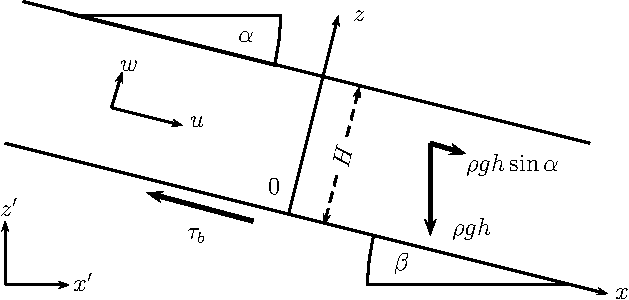
\includegraphics[width=0.7\textwidth]{figures/fig_parallel_slab}

  \caption{Inclined coordinate system for a parallel sided slab.  }
  \label{fig:inclined-slab-coord}
  \index{Mass balance!step climate change}
\end{figure}
%
\paragraph{Body force}
\label{sec:body-force}

In any coordinate system the body force (gravity) is $\mathbf{b}=\rho
\mathbf{g}$.  In the untilted coordinate system $K'$ the body force is
vertical along the $\mathbf{\hat{e}}'_3$ direction
%
\begin{equation}
  \label{eq:body-force}
  \mathbf{b} = - \rho g\, \mathbf{\hat{e}}'_3\,.
\end{equation}
%
The rotation matrix describes the transformation from $K'$ to $K$
%
\begin{equation}
  \label{eq:rotation-matrix}
  \left[ a_{ij} \right] =
  \begin{pmatrix}
    \cos\alpha & 0 & -\sin\alpha \\
    0          & 1 & 0 \\
    \sin\alpha & 0 & \cos\alpha
  \end{pmatrix}
\end{equation}
%
and therefore
%
\begin{align*}
  b_i &= a_{ij} b_j'\\
  \intertext{with the components}
  b_1 &= a_{11} b_1' + a_{12} b_2' + a_{13}b_3'	\\
      &= \cos\alpha \cdot 0 + 0\cdot 0 - \sin\alpha (-g) \\
      &= g\sin\alpha \\
  b_2 &= 0 \\
  b_3 &= -g\cos\alpha\,.    
\end{align*}

\paragraph{Symmetry}
\label{sec:symmetry}

The problem has translational symmetry in the $x$ and $y$ direction.  
It follows that none of the quantities can change in these directions
%
\begin{equation}
  \label{eq:symmetry}
  \frac{\partial \,(\cdot)}{\partial x} = 0 \qquad \text{and} \qquad
  \frac{\partial \,(\cdot)}{\partial y} = 0\,.
\end{equation}
%
Furthermore no deformation takes place in the $y$ direction, i.e.~all
deformation happens in the $x,z$ plane. This is called \emph{plane
  strain}\index{plane strain} and leads to the constraints
%
\begin{equation}
  \label{eq:no-def}
  \epsdot_{yx} = \epsdot_{yy} = \epsdot_{yz} = 0.
\end{equation}

\paragraph{Boundary conditions}
\label{sec:boundary-conditions}

The glacier surface with the face normal $\hat{\mathbf{n}}$ is traction free
%
\begin{equation}
  \label{eq:surface-traction}
  \mathbf{\Sigma}(\hat{\mathbf{n}}) \stackrel{!}{=} \mathbf{0}
  \quad \Longleftrightarrow \quad
  \bsigma \hat{\mathbf{n}} \stackrel{!}{=} \mathbf{0} 
  \quad \Longleftrightarrow \quad
  \bsigma
  \begin{pmatrix}
    0\\0\\1
  \end{pmatrix}
  \stackrel{!}{=} \mathbf{0} 
  \quad \Longleftrightarrow \quad
  \begin{pmatrix}
    \sigma_{xz}\\\sigma_{yz}\\\sigma_{zz}
  \end{pmatrix}
  \stackrel{!}{=} \mathbf{0} \,.
\end{equation}
%
The boundary conditions at the glacier base are $v_x = u_b$, $v_y=0$ and $v_z=0$.

\paragraph{Solution of the system}
\label{sec:solution-system}

We now insert all of the above terms into the field equations
(\ref{eq:mass-continuity-incompressible}) and (\ref{eq:force-balance}). The
mass continuity equation (\ref{eq:mass-continuity-d}) together with
(\ref{eq:symmetry}) leads to
%
\begin{equation}
  0 + 0 + \frac{\partial v_z}{\partial z} = 0.
\end{equation}
%
The velocity component $v_z$ is constant.  Together with the boundary
condition at the base ($v_z=0$) we conclude that $v_z=0$ everywhere.

Most terms in the momentum balance equation (\ref{eq:force-balance-c}) are
zero, and therefore
%
\begin{subequations}
  \begin{align}
    \label{eq:force-balance-slab-a}
    \frac{\partial \sigma_{xz}}{\partial z} &= -\rho g \sin\alpha\,,\\
    \label{eq:force-balance-slab-b}
    \frac{\partial \sigma_{yz}}{\partial z} &= 0\,,\\
    \label{eq:force-balance-slab-c}
    \frac{\partial \sigma_{zz}}{\partial z} &= \rho g \cos\alpha\,.
  \end{align}
\end{subequations}
%
Integration of Equation (\ref{eq:force-balance-slab-a}) and
(\ref{eq:force-balance-slab-c}) with respect to $z$ leads to
%
\begin{align*}
  \sigma_{xz} &= -\rho g z\sin\alpha + c_1,\\
  \sigma_{zz} &= \hspace{1ex}\;\rho g z\cos\alpha + c_2.
\end{align*}
%
The integration constants $c_1$ and $c_2$ can be determined with the traction
boundary conditions (\ref{eq:surface-traction}) at the surface ($z_s=h$) and
lead to
%
\begin{subequations}
  \begin{align}
    \label{eq:stress-slab-depth-a}
    \sigma_{xz}(z) &= \hspace{1ex}\;\,\rho g (h-z)\sin\alpha,\\
    \label{eq:stress-slab-depth-b}
    \sigma_{zz}(z) &= -\rho g (h-z)\cos\alpha.
  \end{align}
\end{subequations}
%
We see that the stresses vary linearly with depth.

To calculate the deformation rates we exploit Glen's Flow Law (\ref{eq:Glen}),
and make use of the fact that the strain rate components are directly related
to the deviatoric stress components.  Obviously we need to calculate the
deviatoric stress tensor \bsigma$^{(d)}$.  Because of the plain strain
condition (Eq.~\ref{eq:no-def}) and the flow law, the deviatoric stresses
in $y$-direction vanish $\sigma^{(d)}_{iy}=0$.  By definition
$\sigma^{(d)}_{yy} = \sigma_{yy}-\sigma_m$ so that $\sigma_{yy} = \sigma_m$,
where use has been made of the definition of the mean stress $\sigma_m :=
\frac{1}{3} \sigma_{ii} = \frac{1}{3}(\sigma_{xx}+\sigma_{yy}+\sigma_{zz})$.

Using again Glen's flow law we also see that (Eq.~\ref{eq:symmetry}a)
%
\begin{equation*}
  \epsdot_{xx} = \frac{\partial v_x}{\partial x} \stackrel{!}{=} 0
  \qquad \text{leads to } \quad \sigma^{(d)}_{xx} = 0
  \qquad\text{and} \quad \sigma_{xx} = \sigma_m. 
\end{equation*}
%
Therefore all diagonal components of the stress tensor are equal to the mean
stress $\sigma_m = \sigma_{xx}=\sigma_{yy}=\sigma_{zz} = -\rho g
(h-z)\cos\alpha$ (using Eq.~\ref{eq:stress-slab-depth-b}).
%
The effective stress $\tau$ can now be calculated with the deviatoric stress
components determined above
%
\begin{align*}
  \sigma^{(d)}_{xx} &= \sigma^{(d)}_{yy} =   \sigma^{(d)}_{zz} = 0,\\
  \sigma^{(d)}_{xy} &= \sigma^{(d)}_{yz} = 0,\\
  \sigma^{(d)}_{xz} &= \rho g (h-z)\sin\alpha,
\end{align*}
%
so that
%
\begin{equation}
  \tau^2 = \frac{1}{2}\sigma^{(d)}_{ij}\sigma^{(d)}_{ij} 
       = \frac{1}{2}\left(2(\sigma^{(d)}_{xz})^2 \right) 
       = (\sigma^{(d)}_{xz})^2 .
\end{equation}
%
With Equation (\ref{eq:stress-slab-depth-a}) we obtain
%
\begin{equation}
\tau = \left|
  \sigma^{(d)}_{xz} \right| = \rho g (h-z)\sin\alpha.
  \label{eq:tau-platte}
\end{equation}

After having determined the deviatoric stresses and the effective stress, we
can calculate the strain rates.  The only non-zero term of the strain rate
tensor is 
%
\begin{align}
  \epsdot_{xz} &= A \tau^{n-1}\sigma^{(d)}_{xz}
  = A \left( \rho g (h-z) \sin\alpha \right)^{n-1}\rho g (H-z) \sin\alpha
  \notag\\
  &= A\left( \rho g (h-z) \sin\alpha \right)^{n}.
\end{align}
\newpage
The velocities can be calculated from the strain rates
%
\begin{equation*}
  \epsdot_{xz} = \frac{1}{2}\left( \frac{\partial v_x}{\partial z} + \frac{\partial v_z}{\partial x} \right)
\end{equation*}
%
where the second term vanishes.  Integration with respect to $z$ leads to
%
\begin{align*}
  v_x(z) &= 2 \int_0^z \epsdot_{xz}(z)\; dz\\
         &= - \frac{2A}{n+1} (\rho g \sin\alpha)^n (H-z)^{n+1} + k
\end{align*}
%
With the boundary condition at the glacier base $v_x(0)=u_b$ we can determine
the constant $k$ as
%
\begin{equation*}
  k = \frac{2A}{n+1} (\rho g \sin\alpha)^n H^{n+1}
\end{equation*}
%
and finally arrive at the velocity distribution in a parallel sided slab
%
\begin{equation}
  \label{eq:parallel-slab-velocity}
 u(z) = v_x(z) = \underbrace{\frac{2A}{n+1} (\rho g \sin\alpha)^n \left( H^{n+1}-(H-z)^{n+1}
  \right)}_{\text{deformation velocity}}\quad + \underbrace{u_b\rule[-1.9ex]{0ex}{1ex}}_{\text{sliding velocity}}
\end{equation}
%
This equation is known as \emph{shallow ice equations}\index{shallow ice equations}, since it
can be shown by rigorous scaling arguments that the longitudinal stress
gradients $\frac{\partial \sigma_{xi}}{\partial x_{i}}$ and $\frac{\partial
  \sigma_{yi}}{\partial x_i}$ are negligible compared to the shear stress for
shallow ice geometries such as the inland parts of ice sheets (except for the
domes).


\section{Flow through a cylindrical channel}
\label{sec:flow-through-cylindrical-channel}

\begin{figure}[bhtp]
  \centering
  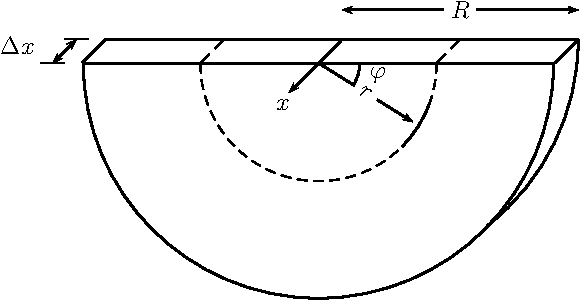
\includegraphics[width=0.7\textwidth]{figures/fig_channel}
  \caption{Coordinate system for a cross section through a valley glacier.  }
  \label{fig:valley-glacier-coord}
\end{figure}

Most glaciers are not infinitely wide but flow through valleys.  The valley
walls exert a resistance, or drag on the glacier flow.  To see how this alters
the velocity field we consider a glacier in a semi-circular valley of radius
$R$ and slope $\alpha$.  The body force from a slice has to be balanced by
tractions acting on the circumference in distance $r$ from the center (in a
cylindrical coordinate system with coordinates $x$, $r$ and $\varphi$)
%
\begin{align}
  \label{eq:force-balance-valley}
  \sigma_{rx} \pi r \Delta x &= -\rho g \frac{\pi r^2}{2} \Delta x\sin \alpha\,, \notag\\
  \sigma_{rx} &= -\frac{1}{2}\, r\, \rho g  \sin \alpha\,. 
\end{align}
%
Since the only non-zero velocity component is in $x$-direction, most
components of the strain rate tensor vanish. Under the assumption of no stress
gradients in $x$-direction and equal shear stress along the cylindrical
perimeter this leads to
%
\begin{align}
  \epsdot_{rr} = \epsdot_{xx} = \epsdot_{\varphi\varphi}= 0 
  \qquad \Longrightarrow \qquad &
  \sigma^{(d)}_{rr} = \sigma^{(d)}_{xx} = \sigma^{(d)}_{\varphi\varphi}= 0  \\
  \text{and also} \qquad & \sigma^{(d)}_{r\varphi} = \sigma^{(d)}_{x\varphi} = 0
\end{align}
%
The second invariant of the deviatoric stress tensor is $\tau =
\left| \sigma_{xr} \right| = \frac{1}{2}r\rho g \sin\alpha$.  To calculate the
velocity we use the flow law (\ref{eq:Glen})
\begin{equation*}
  \frac{1}{2} \frac{d u}{d r} = \epsdot_{xr} = A \tau^{n-1} \sigma_{xr}
  = - A \left( \frac{1}{2} \rho g \sin\alpha  \right)^n r^n
\end{equation*}
%
Integration with respect to $r$ between the bounds $0$ and $R$ gives
%
\begin{equation}
  \label{eq:velo-channel}
  u(0) - u(R) = v_{x}(0) - v_x(R) = 2 A \left( \frac{1}{2}\rho g \sin\alpha \right)^n \frac{R^{n+1}}{n+1}\,.
\end{equation}
%
The channel radius $R$ is equivalent to the ice thickness $H$ in Equation
(\ref{eq:parallel-slab-velocity}) and thus
%
\begin{equation}
  \label{eq:velo-comp-channel-slab}
  u_{\text{def, channel}} = \left( \frac{1}{2} \right)^n   u_{\text{def, slab}}\,.
\end{equation}
%
The flow velocity on the center line of a cylindrical channel is \textbf{eight
  times slower} than in an ice sheet of the same ice thickness.  For further
reference we also write down the velocity at any radius
%
\begin{equation}
  \label{eq:velo-channel-r}
  u(r) = u(0) - 2 A \left( \frac{1}{2}\rho g \sin\alpha \right)^n \frac{r^{n+1}}{n+1}\,.
\end{equation}
%
The ice flux through a cross section is (for $u_R = 0$)
%
\begin{align}
  q = \int_0^R u(r)\, \pi r \, dr
  &= u(0)\, \frac{\pi R^2}{2} - \frac{2 A}{n+1}\left( \frac{1}{2}\rho g
    \sin\alpha \right)^n \pi\int_0^R r^{n+2}\,dr \notag\\
  &= u(0)\, \frac{\pi R^2}{2} - \frac{2}{n+3}\, u(0)\, \frac{\pi R^2}{2} \notag\\
  &= u(0)\, \frac{\pi R^2}{2} \left( 1 - \frac{2}{n+3} \right)
   = u(0)\, \frac{\pi R^2}{2}  \frac{n+1}{n+3}
\end{align}
%
The mean velocity in the cross section is defined by $q = \bar{\bar{u}}\, \frac{\pi
  R^2}{2}$ and is
%
\begin{equation}
  \label{eq:mean-velo-channel1}
  \bar{\bar{u}} = u(0)\, \frac{n+1}{n+3}
\end{equation}
%
The mean velocity at the glacier surface is 
%
\begin{equation}
  \label{eq:mean-velo-channel}
  \bar{u} = \frac{1}{R}\int_0^R u(r)\,dr
  = u(0)\, \frac{2A}{n+1} \left( \frac{1}{2}\rho g \sin\alpha \right)^n
  \frac{R^{n+1}}{n+2}
  = u(0)\, \frac{n+1}{n+2}
\end{equation}

\section{Free Surface}
\label{sec:free-surface}

  \begin{figure}
    \begin{center}
    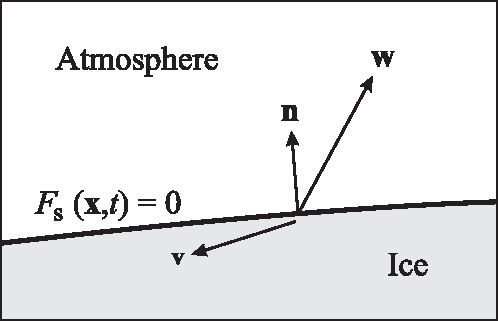
\includegraphics[width=8cm]{figures/fig_5_03}%
    \caption{Geometry of the free surface $F_{\textrm S}(\mathbf{x},t)=0$. $\bn$ is the unit normal vector, $\bv$ is  the ice velocity and $\mathbf{w}$ the velocity of the free surface.}
    \label{fig:free-surface}
  \end{center}
  \end{figure}

The free surface of a glacier can be regarded as a singular surface,
given in implicit form by
\begin{equation} \label{eq:upper-free-surface}
F_{\mathrm{s}}(\mathbf{x},t) = z - h(x,y,t) = 0,
\end{equation} which can be interpreted as a zero-equipotential
surface of the function $F_{\textrm s}(\mathbf{x},t)$, with unit
normal vector
\begin{equation} \label{eq:normal-vector} \bn = \frac{\nabla
F_{\textrm s}}{\vert \nabla F_{\textrm s} \vert},
\end{equation} which points into to atmosphere
(Fig.~\ref{fig:free-surface}), and $\nabla F_{\mathrm s} = (-\partial
h / \partial x, -\partial h / \partial y, 1)$. As a direct consequence
of Eqn.~\eqref{eq:upper-free-surface}, the time derivate of
$f_{\textrm{S}}$ following the motion of the free surface with
velocity $\bw$ must vanish,
\begin{equation} \label{eq:upper-free-surface-derivative}
\DDt{F_{\mathrm s}} = \frac{\partial F_{\mathrm{s}}}{\partial t} + \bw
\cdot \nabla F_{\mathrm S} = 0.
\end{equation} Let $\bv$ be the ice surface velocity, then we can
introduce the ice volume flux through the free surface,
\begin{equation} a_{\mathrm s}^{\perp} = (\bw - \bv)\cdot \bn,
\end{equation} which is the \emph{accumulation-ablation function} or
\emph{surface mass balance}. The sign is chosen such that a supply
(accumulation) is counted as positive and a loss (ablation) as
negative. With this definition and Eqn.~\eqref{eq:normal-vector},
Eqn.~\eqref{eq:upper-free-surface-derivative} can be rewritten as
\begin{equation} \frac{\partial F_{\mathrm{s}}}{\partial t} + \bv
\cdot \nabla F_{\mathrm s} = - \vert \nabla F_{\textrm s} \vert
a_{\mathrm s}^{\perp},
\end{equation} or, by inserting $F_{\mathrm s} = z - h$,
\begin{equation} \label{eq:upper-kinematic-bc} \frac{\partial
h}{\partial t} + v_x \frac{\partial h}{\partial x} + v_y
\frac{\partial h}{\partial y} - v_z = - \vert \nabla F_{\textrm s}
\vert a_{\mathrm s}^{\perp}.
\end{equation} Since this condition has been derived by geometrical
considerations only, it is called the \emph{kinematic boundary
condition}. Provided that the accumulation-ablation function is given,
it evidently governs the evolution of the free surface.

In a similar manner to the upper free surface, a \emph{kinematic
boundary condition} for the ice base can be derived:
\begin{equation} \label{eq:lower-free-surface}
F_{\mathrm{b}}(\mathbf{x},t) = z -b(x,y,t) = 0,
\end{equation} and
\begin{equation} \frac{\partial F_{\mathrm{b}}}{\partial t} + \bv
\cdot \nabla F_{\mathrm b} = - \vert \nabla F_{\textrm b} \vert
a_{\mathrm b}^{\perp},
\end{equation} or, by inserting $F_{\mathrm b} = z - b$,
\begin{equation} \label{eq:lower-kinematic-bc} \frac{\partial
b}{\partial t} + v_x \frac{\partial b}{\partial x} + v_y
\frac{\partial b}{\partial y} - v_z = \vert \nabla F_{\textrm b} \vert
a_{\mathrm b}^{\perp}.
\end{equation}

Now, by combining the continuity equation \eqref{eq:mass-continuity-d}
with the kinematic boundary conditions \eqref{eq:upper-kinematic-bc}
and \eqref{eq:lower-kinematic-bc}, we can derive and evolution
equation for the ice thickness $H(x,y,t) = h(x,y,t)-b(x,y,t)$. First
we integrate \eqref{eq:mass-continuity-d} from the ice base to the
upper surface:
\begin{equation} \int_b^h \left( \frac{\partial v_x}{\partial x} +
\frac{\partial v_y}{\partial y} + \frac{\partial v_z}{\partial z}
\right) \textrm{d}z
\end{equation} Using Leibnitz's rule and
\begin{equation} \int_b^h \frac{\partial w}{\partial z} \textrm{d}z =
w\vert_{z=h} - w\vert_{z=b}
\end{equation} we arrive at
\begin{align} \frac{\partial}{\partial x} \int_b^h v_x \textrm{d}z +
\frac{\partial}{\partial y} \int_b^h v_y \textrm{d}z -
v_x\vert_{z=h}\frac{\partial h}{\partial x}
-v_y\vert_{z=h}\frac{\partial h}{\partial y} + v_z\vert_{z=h}
\nonumber \\ + v_x\vert_{z=b}\frac{\partial b}{\partial x} +
v_y\vert_{z=b}\frac{\partial b}{\partial y} - v_z\vert_{z=b} = 0.
\end{align} With the kinematic boundary conditions
\eqref{eq:upper-kinematic-bc} and \eqref{eq:lower-kinematic-bc}, this
yields
\begin{equation} \frac{\partial\left(h-b\right)}{\partial t} +
\frac{\partial}{\partial x} \int_b^h v_x \textrm{d}z +
\frac{\partial}{\partial y} \int_b^h v_y \textrm{d}z - \vert \nabla
F_{\textrm s} \vert a_{\mathrm s}^{\perp} + \vert \nabla F_{\textrm b}
\vert a_{\mathrm b}^{\perp} = 0.
\end{equation} By introducing the \emph{volume flux} $\mathbf{Q}$ as
the vertically-integrated horizontal velocity, that is
\begin{equation} \mathbf{Q} = \left(
  \begin{array}{c} Q_x \\ Q_y
  \end{array} \right) = \left(
  \begin{array}{c} \int_b^h v_x \textrm{d}z \\ \int_b^h v_y
\textrm{d}z
  \end{array} \right) = \bar \bv H,
\end{equation} where $\bar \bv$ is the depth-averaged velocity. We
obtain
\begin{equation} \frac{\partial H}{\partial t} = - \nabla \cdot
\mathbf{Q} + \vert \nabla F_{\textrm s} \vert a_{\mathrm s}^{\perp} -
\vert \nabla F_{\textrm b} \vert a_{\mathrm b}^{\perp}.
\end{equation} Recall that $a_{\textrm s}^{\perp}$ and $a_{\textrm
b}^{\perp}$ are perpendicular to the free surface and the ice
base. However, since $\frac{\partial H}{\partial t}$ refers to the
vertical direction, we introduce $a_s = \vert \nabla F_{\textrm s}
\vert a_{\mathrm s}^{\perp}$ and $a_b = \vert \nabla F_{\textrm b}
\vert a_{\mathrm b}^{\perp}$, which are in the vertical direction (not
shown, see \cite{GreveBlatter_disg} for a derivation).
\begin{equation} \frac{\partial H}{\partial t} = - \nabla \cdot
\mathbf{Q} + a_{\mathrm s} - a_{\mathrm b}.
\end{equation} This is the ice thickness equation, which is the
central evolution equation in glacier dynamics.

\bibliography{mccarthy}


\end{document}